\section{Świadomie prezentujący ekspert - wyniki}

Podejście \textit{kopiowania zachowań ze świadomie prezentującym ekspertem} nie jest podejściem algorytmicznym. Metoda jest identyczna z \textit{kopiowaniem zachowań}, a jedyną różnicę stanowi zachowanie eksperta podczas generowania trajektorii uczących. Cały przebieg eksperymentu jest identyczny z opisanym w punkcie \ref{bc_results}.
\subsection {Zachowanie eksperta}
Podczas prezentacji ekspert gra tak, żeby na podstawie jego trajektorii mógł zostać utworzony wewnętrznie spójny zestaw danych do nauki. Stara się nie działać na podstawie pamięci, żeby uzasadnienie każdej decyzji mogło zostać wywnioskowane tylko i wyłącznie na podstawie dostępnego klasyfikatorowi stanu. Ekspert dokłada dodatkowych starań, żeby jego działania były spójne, mimo upływającego czasu i wykonywania powtarzalnych czynności. Ekspert generuje i rozwiązuje sytuacje, w których wstępnie nauczony agent nie zachowywał się poprawnie. W szczególności:
\begin{itemize}
\item{w scenariuszu \textit{Trudne zbieranie apteczek} znajdując się w rogu lub na ciasnym zakręcie zawsze wychodzi z niego obracając się w tę samą stronę}
\item{w scenariuszu \textit{Trudne zbieranie apteczek} znajdując się przed miną nie wymija jej, ale w miarę możliwości odwraca się i szuka innej drogi}
\item{w scenariuszu \textit{Obrona środka} pozwala przeciwnikom podejść bliżej (klatki z ,,czekaniem'' nie są brane pod uwagę), żeby zaprezentować zachowanie w otoczeniu przeciwników}
\item{W scenariuszu \textit{Obrona środka} nie odwraca się do zapamiętanych przeciwników, którzy nie są widoczni na ekranie}
\end{itemize}

\subsection{Wyniki}

Przy testowaniu scenariusza \textit{Obrona środka} dla każdej konfiguracji zostało nauczonych 10 agentów, z których każdy został przetestowany odgrywając 10 epizodów. Wynikowa próbka danych składa się ze 100 wyników dla każdej z konfiguracji.

Przy testowaniu scenariusza \textit{Trudne zbieranie apteczek} dla każdej konfiguracji zostało nauczonych od 82 do 111 agentów, z których każdy został przetestowany odgrywając 20 epizodów. Wynikowa próbka danych składa się z od 1620 do 1720 wyników dla każdej z konfiguracji.

W tabelach \ref{tab:presenting_expert_results_dtc} i \ref{tab:presenting_expert_results_hg}  oraz na rysunkach \ref{fig:presenting_expert_results_dtc} i \ref{fig:presenting_expert_results_hg}  przedstawione są wyniki osiągnięte przez agenta w przeprowadzonych eksperymentach.

\begin{figure}[H]
		\ffigbox{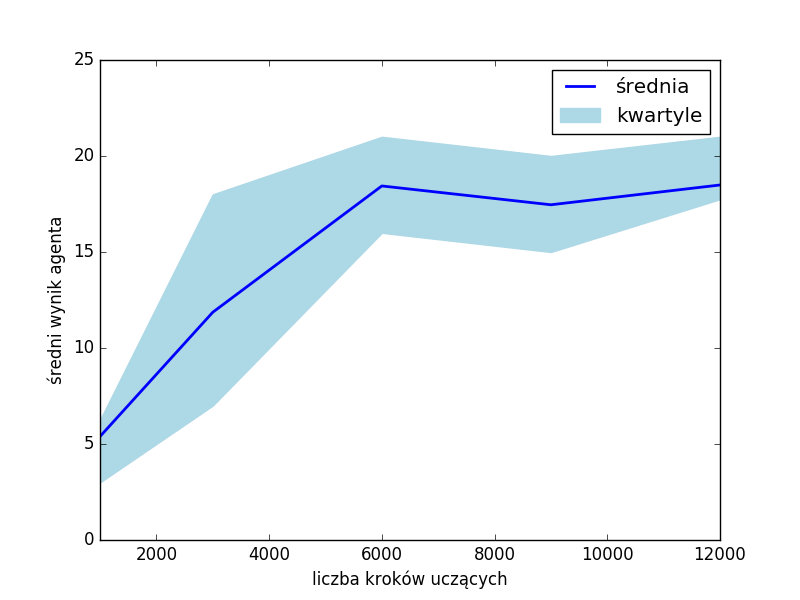
\includegraphics[scale = 0.7]{figures/figures/results/pe_dtc_plot.png}}{\caption{Wyniki agenta nauczonego na podstawie trajektorii \textit{świadomie prezentującego  eksperta} w zależności od liczby kroków uczących w scenariuszu \textit{Obrona środka}}\label{fig:presenting_expert_results_dtc}}
\end{figure}

\begin{figure}[H]
		\ffigbox{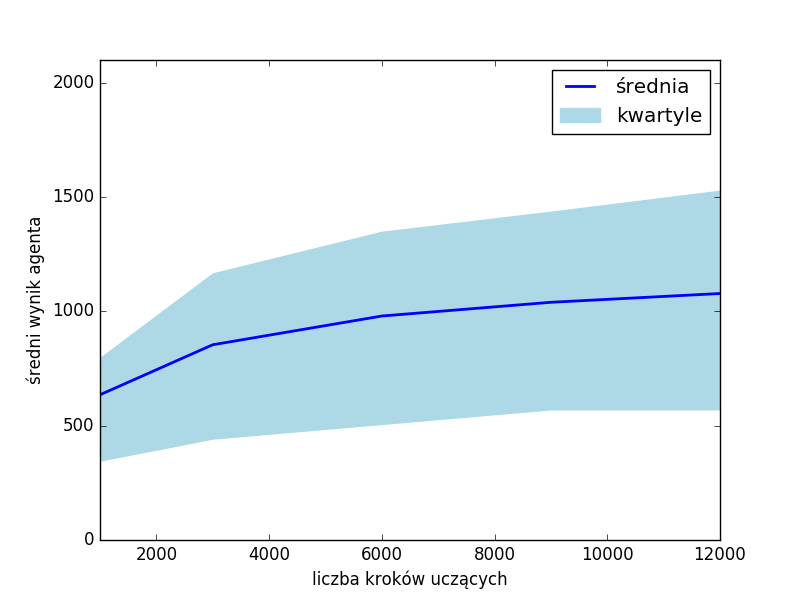
\includegraphics[scale = 0.7]{figures/figures/results/pe_hg_plot.png}}{\caption{Wyniki agenta nauczonego na podstawie trajektorii \textit{świadomie prezentującego  eksperta} w zależności od liczby kroków uczących w scenariuszu \textit{Trudne zbieranie apteczek}}\label{fig:presenting_expert_results_hg}}
\end{figure}

\begin{figure}[H]
\csvautotabular{data/pa_expert_results_dtc.csv}{\caption{Wyniki agenta nauczonego na podstawie trajektorii \textit{świadomie prezentującego eksperta} w zależności od liczby kroków uczących w scenariuszu \textit{Obrona środka}.}\label{tab:presenting_expert_results_dtc}}
\end{figure}

\begin{figure}[H]
\csvautotabular{data/pa_expert_results_hg.csv}{\caption{Wyniki agenta nauczonego na podstawie trajektorii \textit{świadomie prezentującego eksperta} w zależności od liczby kroków uczących w scenariuszu \textit{Trudne zbieranie apteczek}.}\label{tab:presenting_expert_results_hg}}
\end{figure}


\subsection{Zachowanie agenta}
\subsubsection{Trudne zbieranie apteczek}
Agent zachowuje się lepiej, niż odpowiednik nauczony na podstawie normalnych trajektorii.

Problem blokowania się w rogach został w praktyce wyeliminowany. Jedynie w pojedynczych przypadkach agentowi zdarza się zablokować w podobnych, ale nie identycznych sytuacjach i niejednokrotnie agentowi udaje się samemu z nich wydostać.

Mimo wysiłków eksperta nie udało się w zauważalny sposób zmniejszyć problemu wchodzenia w miny.

\subsubsection{Obrona środka}
Agent zachowuje się lepiej, niż odpowiednik nauczony na podstawie normalnych trajektorii.
Osiągane przez niego wyniki znacznie wzrosły, a ich wariancja wyraźnie zmalała, co widać wizualnie w grze agenta. Agent rzadko popełnia wyraźne błędy, a jego niedoskonałości wynikają raczej z suboptymalnego zachowania - decyzje, czy dany przeciwnik powinien zostać zastrzelony czy powinno się go na razie zostawić nie zawsze są podejmowane poprawnie, ale jest to kwestia ,,dostrojenia'' agenta.

\subsection{Analiza i wnioski}

Podejście \textit{kopiowania zachowań ze świadomie prezentującym ekspertem} zgodnie z oczekiwaniami okazuje się skutecznym narzędziem, któremu udało się wyeliminować większość problemów metody bazowej. Eksperymenty potwierdzają hipotezę, że źródłem większości błędów metody \textit{kopiowania zachowań} jest nieumiejętność klasyfikatora do rozróżnienia pewnych klas sytuacji na skutek braku pełnej informacji dostępnej ekspertowi, ale niedostępnej agentowi.

Jedyny problem, którego nie udało się wyeliminować, to wchodzenie w miny w scenariuszu \textit{Trudne zbieranie apteczek}. Zastosowana metoda jest w stanie pokazać, jak agent powinien się zachować w określonej sytuacji, ale nie dostarcza wystarczających narzędzi, żeby pokazać że dane zachowanie jest niepożądane.



